%%%%%%%%%%%%%%%%%%%%% chapter.tex %%%%%%%%%%%%%%%%%%%%%%%%%%%%%%%%%
%
% sample chapter
%
% Use this file as a template for your own input.
%
%%%%%%%%%%%%%%%%%%%%%%%% Springer-Verlag %%%%%%%%%%%%%%%%%%%%%%%%%%
%\motto{Use the template \emph{chapter.tex} to style the various elements of your chapter content.}
\chapter{Elements of Special Relativity}
\label{Relativity} % Always give \ unique label
% use \chaptermark{}
% to alter or adjust the chapter heading in the running 

\section{Introduction}

In 1905 Albert Einstein wrote four papers that would profoundly change physics. The first explained the photoelectric effect, the second was on the Brownian motion, the third stated special relativity and the fourth the equivalence between mass and energy. Each of them were groundbreaking on their own; together, they 
made 1905 be regarded as the {\it Annus Mirabilis} of physics. \\

In this chapter we will discuss the findings of the last two of the four remarkable papers~\cite{Relativity-1,Relativity-2}. As was discussed in Chapter~\ref{chap:Introduction}, special relativity is one of the main pillars of modern physics and in particular of nuclear, subnuclear and elementary particle physics.\\

The first paper was on {\it ``Zur Elektrodynamik bewegter K\"orper''} (``The electrodynamics of moving bodies'') received by {\it Annalen der Physik} on June 30. The second {\it ``Ist die Tr\"gheit eines K\"orpers von seinem Energieinhalt abh\"angig?''} (``Does the Inertia of a Body Depend Upon Its Energy Content?'') was received by the same journal on November 21. \\

\section{Galilean Relativity}

\begin{postulate}[Galilean Relativity]
  \label{postulate:galilean-relativity}
  The laws of mechanics are the same in all inertial reference frames.\\
\end{postulate}

\begin{definition}[Inertial Reference Frame]
  A reference frame in which the 1st law of motion holds exactly (a point-like body without forces acting on it either is still or is moving with constant velocity on a straight line.)
\end{definition}

Starting from the postulate of Galilean Relativity, as an immediate consequence, for an observer in an inertial reference frame it's impossible to determine whether the frame itself is moving or not. \\

\begin{figure}
  \centering
  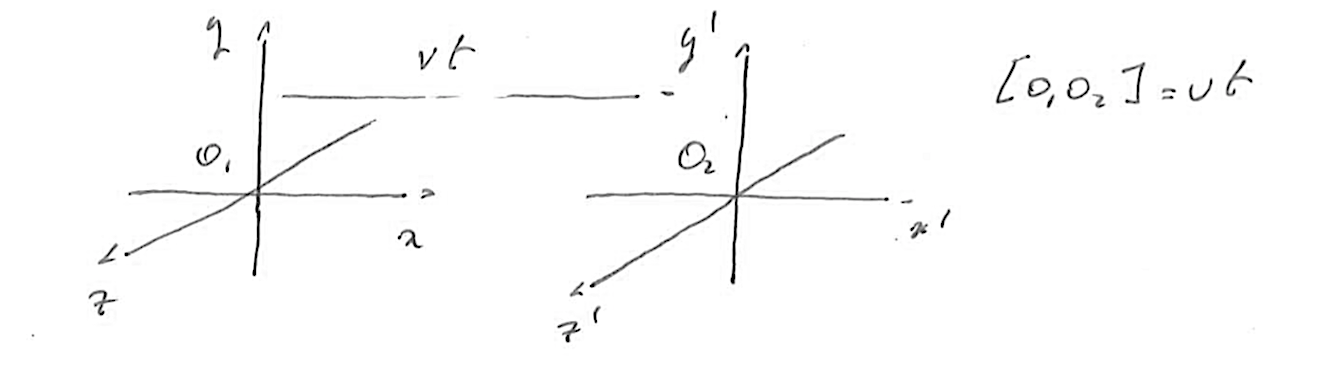
\includegraphics[width=\textwidth]{rel1}
  \caption{An example of an inertial frame $\mathcal{O}'$ moving with respect to another inertial frame $\mathcal{O}$ at constant velocity $v$.}
  \label{fig:rel1}
\end{figure}
A Galilean transformation allows to determine the relation between the coordinates of two inertial reference frames. With reference to Figure \ref{fig:rel1} the relations are the following:

\begin{equation}
  \begin{cases}
    &x = x' + vt\\
    &y = y'\\
    &z = z'\\
    &t = t'\\  
  \end{cases}
  \hspace{2cm}
  \begin{cases}
    x' = x - vt\\
    y' = y'\\
    z' = z\\
    t = t'\\  
  \end{cases}
\end{equation}

The fundamental point in these equations is that the coordinate changes only along the directions for which the components of $\vec{v}$ are different from $0$.\\

The diverging point from Galilean Relativity is an immediate consequence of Maxwell's equations. In fact, it can be easily proven that assuming the validity of Maxwell's equations implies that electromagnetic waves are moving at a constant velocity $c$, \\

\[c\simeq\SI{3e8}{m/s}.\]

At the time of the discovery of Maxwell's equations, physicists were not comfortable with the idea that light, and in general electromagnetic waves, are moving through the void. The common idea at the time was that light is moving through an invisible medium, which is uniformly distributed across the Universe: the \emph{Luminiferous Aether}, or ether. This idea predates modern electromagnetism, and was proposed very early by Christiaan Huygens in his {\it ``Treatise on Light''} in 1690, when he argued that light is a wave that propagates through aether. The concept of "aether" as a general way to explain interactions between bodies and the absence of vacuum was proposed by Robert Boyles a few years earlier. This idea, which was further developed through the years, wasn't fully satisfactory, as it required some sort of imperceptible material. When in the XIX century, with the development of electromagnetism, our knowledge of the nature of light progressed significantly, the existence of a Luminiferous Aether was being very strongly questioned. \\

\section{The Michelson-Morley Experiment}
In order to verify the existence of the Ether, Michelson and Morley developed a particularly sensitive experiment, whose layout is shown in Figure \ref{fig:rel2}. A light beam is produced by a source, and then split by a semi-reflecting mirror into two paths -- one parallel and one orthogonal to the velocity with which the experimental apparatus moves through aether (which is the speed of Earth).

\begin{figure}
  \centering
  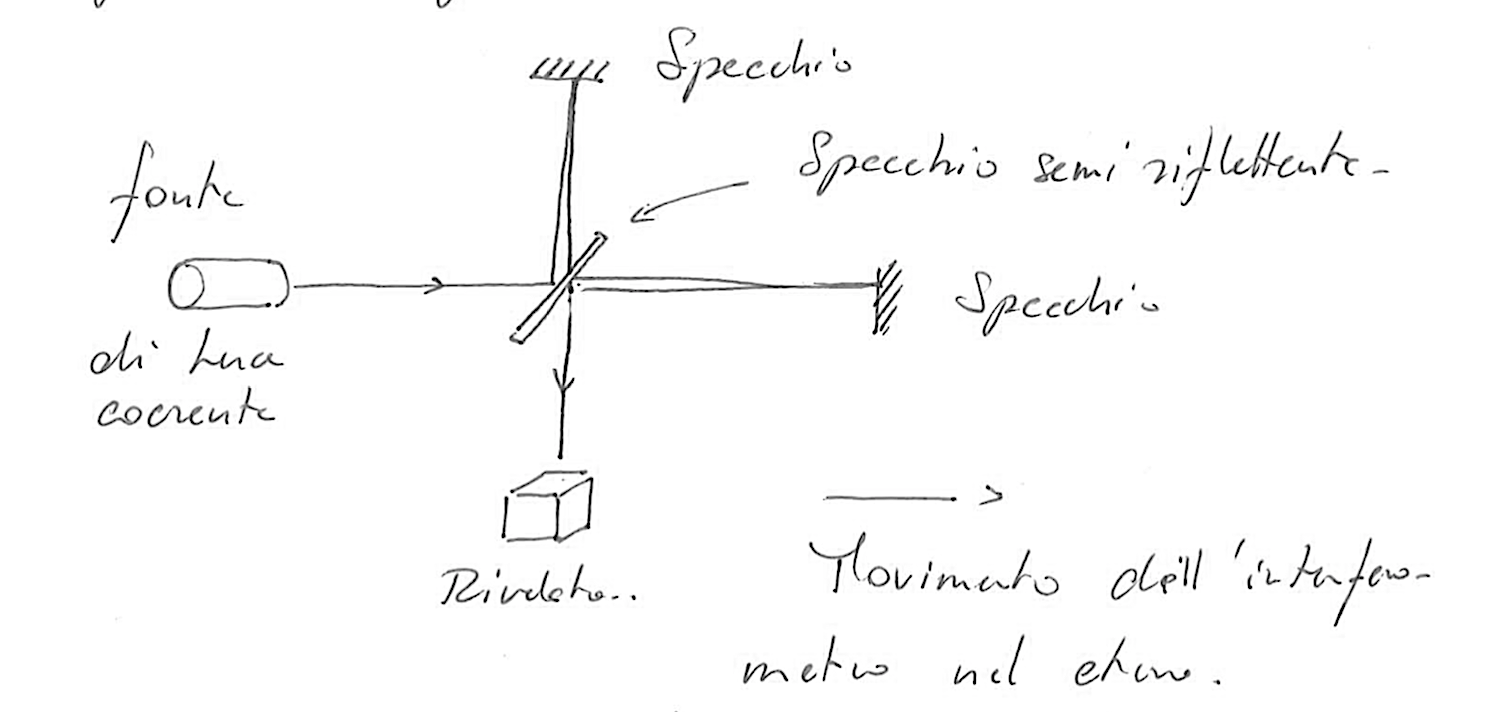
\includegraphics[width=0.8\textwidth]{rel2}
\caption{Layout of Michelson and Morley's experimental apparatus.}\label{fig:rel2}
\end{figure}{}

If the interferometer is moving through aether, then light (which is moving at $c$ with respect to the aether) will travel the distance of the two arms of the spectrometer in a different time, and a corresponding interference pattern will be produced between the two beams.\\

No such interference was visible with the Michelson and Morley experiment: light seemed to travel with the same speed over the two paths. It's only after this unexpected -- yet conclusive -- experimental result that physicists started to reject the idea of aether, accepting the fact that light travels at the same speed in all reference frames. \\

\section{From Simultaneity to Lorentz Transforms}
The theory of \emph{Special Relativity} is the theory which aims at describe space (and time) transformations between two inertial reference frames, one of which is moving with a constant velocity $\vec{v}$ with respect to the other.\\

The foundation of Special Relativity is on the following postulate, which is considered in addition to Postulate \ref{postulate:galilean-relativity}.

\begin{postulate}[Invariance of $c$]
  \label{postulate:invariance-of-c}
  The speed of light $c$ has the same value in all inertial reference frames. Its value is equal to
  \[c = \SI{299792458}{m/s}.\]
\end{postulate}

The theory of Special Relativity was built by Albert Einstein, starting from these two postulates, and exploiting more deeply the concept of \emph{Simultaneity}.
Einstein's definition of simultaneity follows from the following example. Consider two events which happen in two different points of the coordinate space: the two events can be considered as simultaneous if, after each one of them emits a light beam directed to the other event's position, an observer which is in the middle of them sees both the light beams at the same time.\\

\begin{figure}
  \centering
  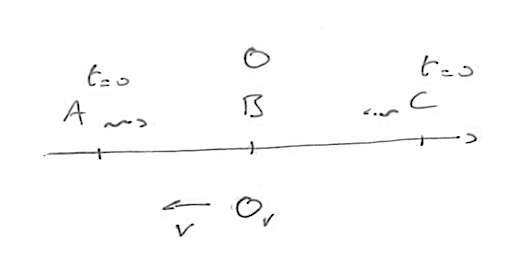
\includegraphics[width=0.8\textwidth]{rel3}
\caption{Graphic representation of simultaneity}  \label{fig:rel3}
\end{figure}{}

Let's make a more detailed overview of this example. With reference to figure \ref{fig:rel3}, an observer $O$ which is in $B$, whose position is fixed with respect to $A$ and $C$, will see the light from $A$ and $C$ simultaneously. Instead, an observer $O'$ which is moving with constant velocity $\vec{v}$ will see the light from $A$ before the light coming from $C$. In general, we have to take into account the fact that simultaneity depends on the reference frame!\\

Let's consider the example in a quantitative way: we want to find the coordinates of two events which are simultaneous by hypothesis (light beams from $A$ and $C$ reach the observer in $B$) in the moving reference frame $O'$. We call the space and time axes of $O'$ as $(x,t)$, which define the plane shown in Figure \ref{fig:rel4}: on this plane, the equation of motion of a light beam is a straight line with slope $t/x=1/c$ or $t/x=-1/c$ -- depending the direction along which it is emitted. The point $B$ lies on the same line as $A$ and $C$, at a distance $l$ from either. We call instead $(x', y')$ the coordinate system as measured by the observer in $O=B$.

\begin{figure}
  \centering
  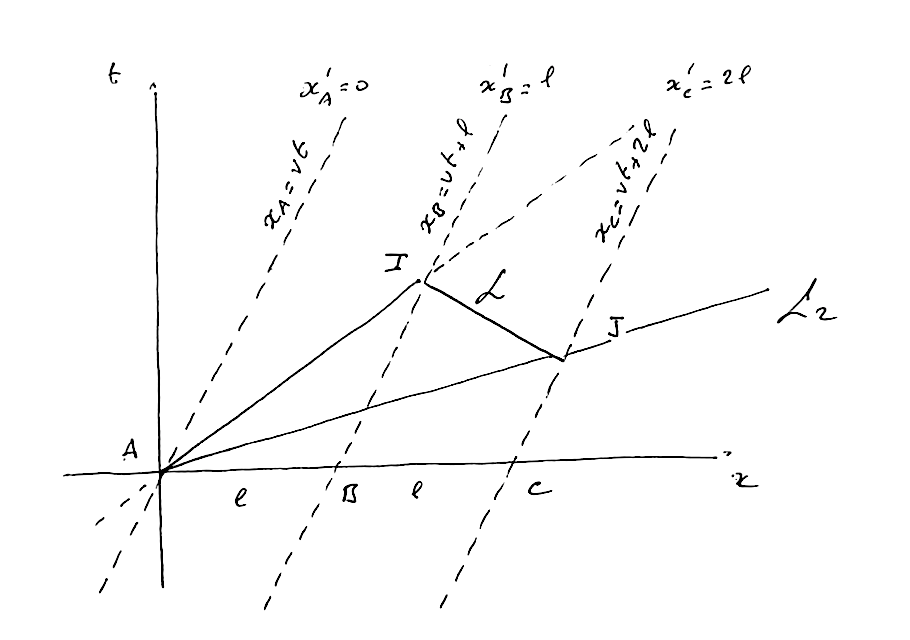
\includegraphics[width=0.8\textwidth]{rel4}
  \caption{In this figure, the coordinates $(x,t)$ belong to the reference frame of $O'$, which is moving at constant velocity $\vec{v}$ with respect to the points $A$, $B$ and $C$. Coordinates $(x',t')$ are the coordinates of the observer $O$, fixed with respect to $A$, $B$ and $C$.}  \label{fig:rel4}
\end{figure}

Let's compute the coordinates $(x_I,t_I)$ of the event $I$, ``Beam from $A$ arrives in $B$''. The point $A$ moves with constant speed $v$ with respect to $O'$, so the coordinates of $I$ will follow the equation of motion
\[x_I=vt_I+l.\]
But the beam moves with speed $c$, so
\[x_I=ct_I,\]
and hence
\[vt_I+l=ct_I,\]
which leads us to
\begin{align}
  t_I&=\frac{l}{c-v},\\
  x_I&=ct_I=\frac{cl}{c-v}.
\end{align}
In order for the event ``Beam from $A$ arrives in $B$'' to be simultaneous with the event ``Beam from $C$ arrives in $B$'', in the reference frame $O'(x,t)$ the second beam must have been emitted in point $J$, i.e. at a time $t_J\neq0$. This beam will travel in the direction of negative $x$, following the equation of motion
\[x=-ct+\alpha,\]
which corresponds to the line $\mathcal{L}$ on the $(x,t)$ plane of Fig. \ref{fig:rel4}; $\alpha$ is an unknown.
Since the second beam does reach the first beam in the intersection point $I$, then also the $I$ should satisfy the same equation,
\[x_I=\frac{cl}{c-v} = -\frac{cl}{c-v} + \alpha,\]
from which one has
\[\alpha = \frac{2cl}{c-v} = \frac{2l}{1-\frac{v}{c}},\]
and by defining
\begin{equation}
  \label{eq:beta}
  \beta = \frac{v}{c}
\end{equation}
we finally obtain
\begin{equation}
  \mathcal{L}:\ \ x=-ct+\frac{2l}{1-\beta}.
\end{equation}

The point $J$ has coordinates
\[
x_J = vt_J+2l,
\]
since it represents the position on the $(x,t)$ plane of the light source in $C=(l, 0)$ after a time $t_J$ has elapsed. It must also satisfy the equation for $\mathcal{L}$, so
\begin{align*}
  x_J = vt_J+2l &= -ct_J+\frac{2l}{1-\beta},\\
  \left[v+c\right]t_J &= 2l \left[\frac{1}{1-\beta}-1\right],\\
  c\left[1+\beta\right]t_J &= 2l \left[\frac{1-1+\beta}{1-\beta}\right],\\
  \left[1+\beta\right]t_J &= \frac{2l}{c} \left[\frac{\beta}{1-\beta}\right],\\
\end{align*}
which gives us
\begin{equation}
  t_J =\frac{2l}{c}\,\frac{\beta}{1-\beta^2},
\end{equation}
and
\begin{equation*}
    \begin{split}
  x_J &= vt_J+2l\\
  &= 2l \frac{\beta^2}{1-\beta^2} + 2l\,\frac{1-\beta^2}{1-\beta^2}\\
  &= 2l \frac{1}{1-\beta^2}\\
  &= \frac{c}{\beta}\,t_J,
  \end{split}
\end{equation*}
which is also the equation for the line $\mathcal{L}_2$. Each point on $\mathcal{L}_2$ corresponds to a simultaneous event.\\

The next task is then to derive the correct transformation laws which allow us to go from the coordinates $(x,t)$ to $(x',t')$. If $x = vt$ then the coordinate $x'$ should be zero (as $v$ is the speed of $O'(x,t)$ with respect to $O(x',t')$). This implies that
\[x' = f(v)\cdot(x-vt).\]

At this point it is important to note that events on the line $\mathcal{L}_2$ correspond to points that are \emph{simultaneous}. It is then explicit that {\bf simultaneity is frame dependent}. In the moving frame the events $A$ occurring at $t=0$ (see Fig.~\ref{fig:rel4}) and the event $J$ are not occurring at equal times, but \emph{they are simultaneous} from the Einstein light-ray definition of simultaneity. This also means that the time of event $J$ in the rest frame of the points $A$, $B$ and $C$ corresponds to $t'=0$. The line $\mathcal{L}_2$ therefore corresponds to $t'=0$.

For this reason, from the parametric form of $\mathcal{L}_2$, $t = xv/c^2 $, the following functional form is expected for $t'$:

\[t' = g(v)\cdot\left(t-\frac{v}{c^2}x\right)\]

Continuing on the {\it gedanken} experiment, let's suppose we consider a point along the the light ray emitted at $t=0$ at point A, whose spatial coordinates will therefore be $x=ct$. Since $A$ is part of $\mathcal{L}_2$, it also has $t'=0$, and since the light is assumed to be propagating at the same speed $c$ in any reference frame, then one has 
\begin{equation}
  \label{eq:B:1}
     x = ct \Rightarrow
    x'=ct'.
 \end{equation}
Using this necessary condition in the previous equations, we straightforwardly obtain that:
\begin{eqnarray*}
  x' &=& (x-vt)\cdot f(v) = (ct-vt)\cdot f(v)\\
  &=& t(c-v)\cdot f(v),\\
  t' &=& \left(t-\frac{v}{c}t\right)\cdot g(v)\\
  &=& \frac{1}{c} (c-v) t \cdot g(v)\\
  &=& \frac{1}{c} x' \frac{g(v)}{f(v)},
\end{eqnarray*}
from which one can deduce that the equation \eqref{eq:B:1} is satisfied if and only if:
\[g(v) = f(v).\]

To further derive the form of the coordinates transformations, another important {\it gedanken} step has to be taken. If the laws of physics are invariant in any inertial reference frame, then there is no difference in considering the expression of coordinates $(x',t')$ as function of $(x,t)$ or \emph{vice versa}. The expression of $(x,t)$ as function of $(x',t')$ should have the same functional form, but with an opposite velocity terms:

\begin{equation}
  \begin{cases}
    x = (x'+vt')f(v),\\
    t = \left(t' + \frac{v}{c^2}x\right)f(v),
  \end{cases}
\end{equation}
and substituting the expression for $x'$ one gets
\begin{eqnarray*}
  x &=& \left[ \left( x-vt\right)f(v)+\left(vt-\beta^2x\right)f(v)\right]f(v)\\
  &=& x\left[f(v)^2\left(1-\beta^2\right)\right].
\end{eqnarray*}
We can then define
\begin{equation}
  \label{eq:gamma}
  \gamma = f(v) = \frac{1}{\sqrt{1-\beta^2}},
\end{equation}
and express the Lorentz transformations as
\begin{eqnarray}
  x' &=& \frac{x-vt}{\sqrt{1-\frac{v^2}{c^2}}},\\
  t' &=& \frac{t-\frac{v}{c^2}x}{\sqrt{1-\frac{v^2}{c^2}}}.\\
\end{eqnarray}
or, using \eqref{eq:beta} and \eqref{eq:gamma}:
\begin{eqnarray}
  x' &=& \gamma x -\beta\gamma c t \\
  ct' &=& \gamma ct -\beta\gamma x
\end{eqnarray}
Note that $\beta\leq1$, $\gamma\geq1$

Note that in the limit $v/c \ll 1$ the Galilean expression of coordinate transformations is recovered. If we consider a Lorentz transformation in three dimensions, we can always make a rotation of the reference frame which brings our coordinate system with an axis ($x$ for example) parallel to $\vec{v}$. Then, the coordinates along axes which are orthogonal to the  direction of motion will not be affected by the transformation. 

The transformation can then be written as
\begin{equation}
  L(\beta)=
  \begin{bmatrix}
    ct'\\
    x'\\
    y'\\
    z'
  \end{bmatrix}
  =
  \begin{bmatrix}
    \gamma & -\beta\gamma & 0 & 0\\
    -\beta\gamma & \gamma & 0 & 0\\
    0 & 0 & 1 & 0\\
    0 & 0 & 0 & 1  
  \end{bmatrix}
  \begin{bmatrix}
    ct\\
    x\\
    y\\
    z
  \end{bmatrix},
\end{equation}

Note that the matrix is a symmetrical diagonalizable block matrix, and also:
\begin{equation}
  \det(L\left(\beta)\right) = \gamma^2 - \beta^2\gamma^2 = 1.
\end{equation}

As a simple consequence of the invariance of reference frames, the inverse matrix will be the one which describes the transformation from $(ct',x',y',z')$ coordinates to $(ct,x,y,z)$, i.e. the same matrix with a positive sign in front of $\beta$.

\begin{equation}
  L^{-1}(\beta)=
  \begin{bmatrix}
    \gamma & \beta\gamma & 0 & 0\\
    \beta\gamma & \gamma & 0 & 0\\
    0 & 0 & 1 & 0\\
    0 & 0 & 0 & 1  
  \end{bmatrix}.
\end{equation}

In the non-relativistic approximation it is common to consider the following expansion:
\begin{equation}
  \gamma = 1 + \frac{\beta^2}{2}+\mathcal{O}(\beta^2),
\end{equation}
which gives:
\begin{eqnarray*}
  x' &= & \gamma\left(x-\beta c t\right) = \left(1+\frac{\beta^2}{2}\right)\left(x-\beta c t\right)\\
  &= &x - \beta c t +\mathcal{O}(\beta^2),\\
  &\sim & x - vt,
\end{eqnarray*}
and
\begin{eqnarray*}
  t' &=& \gamma t -\frac{1}{c}\beta\gamma x \\
  &=& \left(1+\frac{\beta^2}{2}\right) t - \frac{\beta}{c}\left(1+\frac{\beta^2}{2}\right) x \\
  &=& t - \frac{\beta}{c}x +\mathcal{O}(\beta^2)\\
  &=& t - \frac{\beta^2}{v}x +\mathcal{O}(\beta^2)\\
  &\sim & t.
\end{eqnarray*}
As expected, we obtain Galilean transformations.\\

It is interesting to note that Lorentz transformations define a symmetry in 4-dimensional space. Other typical phenomena of Special Relativity can be derived from the structure of coordinate transformations.

\subsection{Contraction of lengths}
When we measure the length of an object, for example with a ruler, what we are measuring is the distance between its two endpoints, $A$ and $B$, i.e. we are measuring two positions. As the object may be moving with respect to us, we need to make sure we perform these two position measurements at the same time (in our reference frame).

\begin{figure}
  \centering
  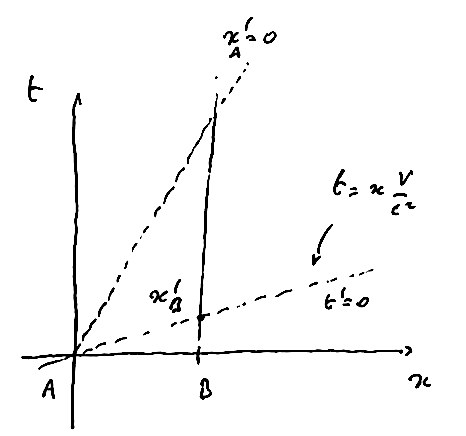
\includegraphics[width=0.8\textwidth]{rel5}
  \caption{Contraction of lengths between  two reference systems}
  \label{fig:rel5contraction}
\end{figure}{}

Figure~\ref{fig:rel5contraction} shows the position of the points $A$ and $B$ of an object in the reference frame $O(x,t)$. Since we have taken (with no loss of generality) $x_A=0$, the length of the object will be
\[L=x_B-x_A=x_B.\]
In the reference frame $O'(x',t')$, which moves with respect to $O$ with a speed $v=\beta c$, we will have
\begin{align*}
x'_A&=\gamma\left(x_A-vt_A\right) = -vt_A,\\
x'_B&=\gamma\left(x_B-vt_B\right).
\end{align*}
We perform the two measurements at the same time $t_A'=t_B'$, and we can take (with no loss of generality) $t_A'=0$. Therefore,
\begin{align*}
t_A&=\gamma(x_A\frac{v}{c^2}+t_A')=0,\\
t_B&=\gamma(x_B\frac{v}{c^2}+t_B') = \gamma x_B \frac{v}{c^2},
\end{align*}
and so
\begin{align*}
x'_A &= -vt_A=0,\\
x'_B &= \gamma x_B \left(1-\frac{v^2}{c^2}\right) = \gamma x_B (1-\beta^2)= x_B \frac{1}{\gamma} ,\\
\end{align*}
which leads to
\begin{equation}
  L' = x_B'-x_A'=\frac{L}{\gamma}.
\end{equation}
This means that the distance in the $O'$ frame is reduced by a factor $1/\gamma$. In a very similar way it is possible to compute that the distance measured by an observer in the $O$ frame is also reduced by the same factor.

\subsection{Time dilation}
Measuring time intervals in a given reference frame requires a clock to be put in a known, fixed position in that reference frame. For example, if we are at a Formula 1 race and we want to measure the distance between the events "first car reaches the finish line" and the event "second car reaches the finish line", we will place a clock at the finish line and read out its two measurements: their difference will be the desired time interval.

Let us consider the sketch in Fig. \ref{fig:rel6}. We are in the reference frame $O(x,t)$, and place a clock in point $A$ which (with no loss of generality) has $x=0$. We take a first time measurement $(x_1=0,t_1)$ (first car reaches $A$), and then another one $(x_2=,t_2)$ (second car reaches $A$). We have
\[
\Delta t = t_2 - t_1,
\]
and we want to measure $\Delta t'$ in a moving reference frame $O'$ (a third car).

\begin{figure}
  \centering
  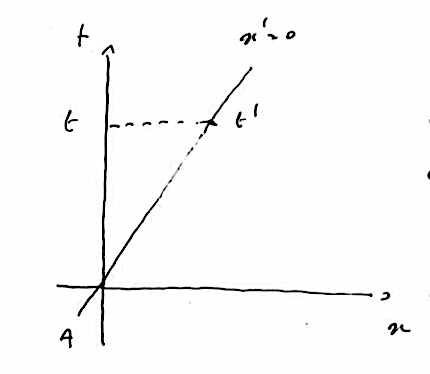
\includegraphics[width=0.8\textwidth]{rel6}
  \caption{Dilation of time between two reference systems}
    \label{fig:rel6}
\end{figure}{}

From the Lorentz transformations, we have
\begin{align*}
    t_1' = \gamma\left(t_1-\frac{\beta}{c}x_1\right),\\
    t_2' = \gamma\left(t_2-\frac{\beta}{c}x_2\right).\\
\end{align*}
The key point here is that the time measurement in $O$ must be performed keeping the clock in the same, fixed position $x_1=x_2$. Therefore, one gets immediately
\begin{equation}
  \Delta t' = \gamma \Delta t,
\end{equation}
a result known as \emph{time dilation}. In other words, the time interval between two events which happen at the same place in one reference system is always lower than measured by a moving reference frame. Note that this result is independent on the direction of velocity, and is the principle on which the so-called \emph{Twin Paradox} is built.\\

\subsection{Metrics}
Since the Lorentz transformations contract distances and dilate time intervals, one would expect the space-time distance to be preserved. Let's see if this is the case.

Consider a point $(x,t)$ and its Lorentz-transformed $(x',t')$:
\begin{align*}
  x' &= \gamma \left(x-\beta c t\right),\\
  t' &= \gamma \left(t-\frac{\beta}{c} x\right).
\end{align*}
By squaring both equations, we get
\begin{eqnarray*}
  x'^2 &=& \gamma^2 \left(x-\beta c t\right)^2\\
  &=& \gamma^2 \left(x^2 + \beta^2c^2t^2 -2\beta c x t\right),\\
  t'^2 &=& \gamma^2 \left(t-\frac{\beta}{c} x\right)^2\\
  &=& \gamma^2 \left(t^2+\frac{\beta^2}{c^2} x^2 -2\frac{\beta}{c}xt\right),\\
\end{eqnarray*}
so that
\begin{eqnarray*}
  (ct')^2&=& \gamma^2 \left((ct)^2+\beta^2 x^2 -2\beta x (ct)\right),\\
  x'^2  &=& \gamma^2 \left(x^2 + \beta^2(ct)^2 -2\beta x (ct)\right).\\
\end{eqnarray*}

It is clear that the distance $(x^2+t^2)$ does not work, because it's not conserved by Lorentz transformation. Instead, the distance defined as $(ct)^2 - x^2$ is conserved:
\begin{eqnarray*}
  (ct')^2 - x'^2 &=& \gamma^2\left[(ct)^2(1-\beta^2) + x^2(\beta^2 -1 ) \right]\\
  &=& \gamma^2 \left[(ct)^2-x^2\right](1-\beta^2)\\
  &=& (ct)^2 - x^2.\\
\end{eqnarray*}
The extension of this result to transformation with three components of velocity is trivial, where the distance $(ct)^2 - x^2 - y^2 -z^2$ is conserved. In other words, the following quantity is a relativistic invariant:
\begin{equation}
  \Delta s^2 = c^2 \Delta t^2 - \Delta x^2 - \Delta y^2 -\Delta z^2,
\end{equation}
or, better, in infinitesimal form:
\begin{equation}
  \dif{s}^2 = c^2 \dif{t}^2 - \dif{x}^2 - \dif{y}^2 -\dif{z}^2.
\end{equation}


\subsection{Proper time}
Consider again a clock which is moving together with an observer, as in Fig. \ref{fig:rel6}. In its reference frame $O'$, one has that $\dif{x}=\dif{y}=\dif{z}=0$ by construction (a reference frame is at rest with respect to itself). So we get
\[\dif{s}^2=c^2\dif{t}^2 - \dif{x}^2 - \dif{y}^2 - \dif{z}^2 = c^2 \dif{s}' = c^2 \dif{t}'^2\]
Thus, one can define the \emph{proper time}
\[
\dif{\tau} = \frac{\dif{s}}{c},
\]
which has the meaning to a metric measure of space-time, also called Minkowski space-time\footnote{You will appreciate the difference between Minkowski space-time and space-times which stem from different assumptions on how $\dif{s}$ depends on $\dif{x}, \dif{y}, \dif{z}, \dif{t}$ when studying general relativity.}.

\subsection{Light Cone}
Let us now consider the trajectory of a particle in space--time. In general, the trajectory of a particle always defines a time--like interval.
\begin{figure}
  \centering
  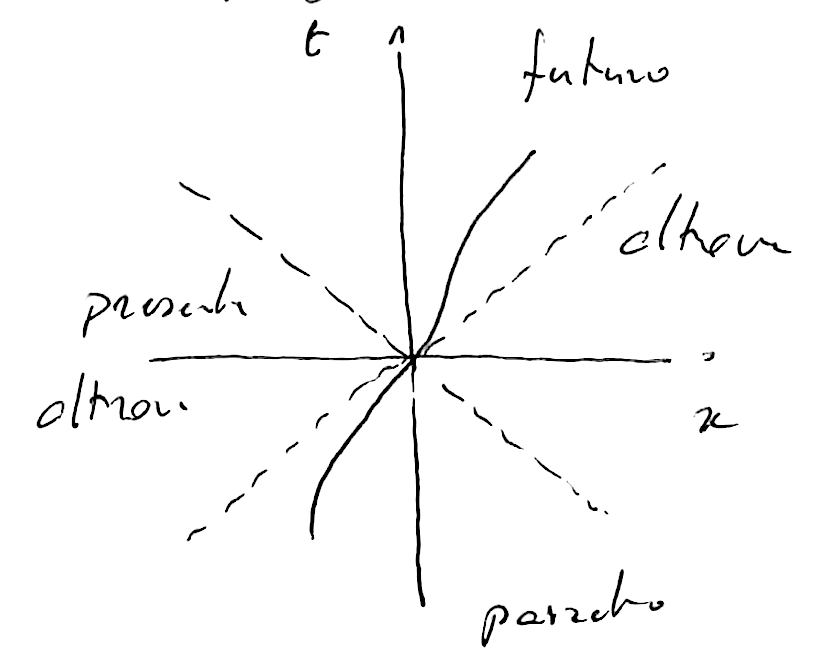
\includegraphics[width=0.5\textwidth]{rel7}
  \caption{Schematic representation of the light cone}\label{fig:rel7}
\end{figure}

\begin{definition}[Time--like interval]
  A time--like interval is a segment in space-time which satisfies:
  \[\dif{s}^2 = \left(c \dif {t}\right)^2 - \left(\dif{\vec{r}}\right)^2 > 0.\]
\end{definition}
For each time--like interval one can always write a corresponding Lorentz transformation for which $\dif{\vec{r}} = \vec{0}$, i.e. there is an inertial reference frame for which the two events are happening in the same place (at different times).

\begin{definition}[Space--like interval]
  A space--like interval is a segment in space-time which satisfies
  \[\dif{s}^2 = \left(c \dif{t}\right)^2 - \left(\dif{\vec{r}}\right)^2 < 0.\]
\end{definition}
In this case it's always possible to write a Lorentz transformation for which $\dif{t} = 0$, i.e. there is an inertial reference frame for which the two events are happening at the same time (in different places).\\

The space-time region in which $\dif {s}^2 = 0$ defines the \emph{light cone}. Events which are inside the light cone can belong to the past, present or future, and they can be connected with a time-like segment to the origin: in other words, they can be connected with a trajectory.

Events outside the light cone can be connected to the origin only with a space-like segment. This implies that a point outside the light cone can not be causally related.

\section{Four-vectors and covariant Notation}\label{sec:covariant1}
We have already introduced four--vectors: $(ct,x,y,z)$. Let's now introduce four-vectors with the superscript notation, which expresses each of its components in a short form:
\[x^\mu = \left(ct,x,y,z\right).\]

The position of the index (superscript or subscript) matters! The corresponding four-vector $x_\mu$ is defined as:
\[x_\mu = \left(ct,-x,-y,-z\right)\]

The action of ``moving the index from upper to lower position'' corresponds to the action of putting a minus sign in front of spatial coordinates. In other words, it corresponds to the multiplication of the four-vector by the \emph{metric tensor} $g^{\mu\nu}$, defined as\footnote{General relativity will show you why we took the disturb to use a tensor to describe operations, like computing $\dif{s}$, which are somehow simple: what here seems useless will prove crucial to deal elegantly with space-times more complex than the Minkowski space-time.}:
\begin{equation}
  g^{\mu\nu}=
  \begin{pmatrix}
    1 & 0 & 0 & 0  \\
    0 & -1 & 0 & 0  \\
    0 & 0 & -1 & 0  \\
    0 & 0 & 0 & -1  
  \end{pmatrix}.
\end{equation}
From this moment, we will also assume the convention of leave out sums on repeated indices: this is a common way to manipulate four-vectors also known as \emph{Einstein notation}. For example, the application of the tensor $g^{\mu\nu}$ to the four-vector $x_\nu$ can be written as:
\[x^{\mu} = \sum_{\nu=0}^3 g^{\mu\nu}x_\nu \equiv g^{\mu\nu}x_\nu.\]

Using the Einstein notation, the product between two four--vectors $U$ and $V$ can be written as:
\[U^\mu V_\nu = U^0V^0 - U^1V^1 - U^2V^2 - U^3V^3\]
and the Lorentz invariant $\Delta s^2$ can be written as:
\[\Delta s^2 = \Delta x^\mu \Delta x_\mu \]
Now, if we compute the differential of the four--vector $x^\mu = (ct, x, y, z)$, we obtain:
\begin{eqnarray*}
  \dif{x}^\mu &=& (c \dif{t}, \dif{x},\dif{y},\dif{z})\\
  \dif{s}^2 &=& \dif{x}^\mu \dif{x}_\mu
\end{eqnarray*}

As we have seen, proper time is defined as follows:
\begin{eqnarray*}
  d\tau^2 &=& \dif{t}^2 - \frac{1}{c^2}\left(\dif{x}^2+\dif{y}^2+\dif{z}^2\right),\\
  d\tau &=& \dif{t}\,\sqrt{ 1 - \frac{1}{c^2}\left(v_x^2+v_y^2+v_z^2\right)},\\
  d\tau &=& \dif{t}\,\sqrt{ 1 - \beta^2},\\
  d\tau &=& \frac{\dif{t}}{\gamma}.
\end{eqnarray*}

Velocity is clearly not invariant under Lorentz transformations, but we can  define the four-velocity as:
\begin{equation}  
u^\mu = \frac{\dif{x}^\mu}{d\tau},
\end{equation}  
which \emph{is} Lorentz-invariant.

It is a common convention to use $\mu$, $\nu$ and other Greek characters for indices running over the four components of four-vectors. To avoid errors, we will adopt the following two notational conventions, widely used in modern physics textbooks and literature:
\begin{itemize}
\item Four--vectors in space--time are denoted only and always with Greek indices, e.g. $x^\mu = (cx_0,x_1,x_2,x_3)$;\\
\item Three--vectors in three dimensional space are only and always written with latin indices, e.g. $x^j = (x_1,x_2,x_3)$.
\end{itemize}
This is equivalent to say that Greek indices range from $0$ to $3$, and latin ones from $1$ to $3$.

For example, we will denote velocity in space (three--vector) with:
\[\vec{v} = (v^1,v^2,v^3) = \left(\frac{\dif{x}_1}{\dif{t}},\frac{\dif{x}_2}{\dif{t}},\frac{\dif{x}_3}{\dif{t}}\right) \equiv v^i.\]

Following the definition of four-velocity:
\begin{eqnarray*}
  u^i &=& \frac{\dif{x}_i}{d\tau}\\
  &=& v_i\, \frac{\dif{t}}{d\tau},
\end{eqnarray*}
which allows us to write the common expression of four--velocity:
\begin{equation}
u^\mu = \gamma (c, \vec{v}),
\end{equation}
which highlights the definition of four-velocity as the proper-time derivative of a space-time four-vector. Although four-velocity is a four-vector, it has only three independent components due to the definition of $\gamma$, which immediately relates $u^0$ and $u^i$.

Motion and trajectories in space-time are defined in terms of $x^\mu$ and $u^\mu$, as illustrated in Fig. \ref{fig:rel8}.
\begin{figure}
  \centering
  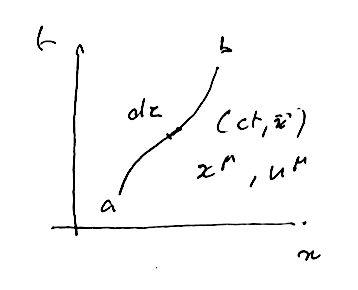
\includegraphics[width=0.5\textwidth]{rel8}
  \caption{Example of trajectory in a Minkowski space in terms of $x^\mu$ and $u^\mu$ }\label{fig:rel8}
\end{figure}

%\section{The Principle of Least Action in Non Relativistic Mechanics}

\section{Relativistic action and Hamiltonian of a particle}
To determine the dynamics of a system in this new relativistic framework a powerful starting point is the principle of least action, from which the Lagrangian and Hamiltonian describing the evolution of the system can be derived, as well as the equations of motion of a relativistic free particle. 

Action, as in classical mechanics, has to be constructed from the trajectory of a particle and {\it should} be invariant under Lorentz transformations. The latter condition ensures the principle of relativity, that the laws of physics are independent of the inertial reference frame we choose to describe them in. 

\begin{note}
The Galilean invariance of the action in Newtonian mechanics is not trivial, while it is straightforward from the fundamental principle of dynamics that Newtonian mechanics is invariant under Galilean transformations. Constructing the free particle action, both in the relativistic and Newtonian mechanics, imposing isotropy and homogeneity of space and time translation invariance of forces, the Lagrangian can only be a function of the square of the velocity of the particle, $\mathcal{L}(\vec{x},\vec{v},t) = \mathcal{L}(v^2)$. A Galilean transformation with a constant velocity $\vec{u}$ will transform $\vec{v} \rightarrow \vec{v} + \vec{u}$ and therefore $ v^2 \rightarrow v^2 + u^2 + 2\vec{v}.\vec{u}$. In this case it appears that if the Lagrangian is linear in $v^2$, then applying the Euler--Lagrange equations, the equations of motion will be invariant under a Galilean transformation. However, here the action is not explicitly invariant under Galilean transformations, but the equations of motion are. From this, it is also apparent that if the Lagrangian is not a linear function of $v^2$ then the equations of motion will not be invariant.
\end{note}

The only invariant we have built from the trajectory of a particle is the proper time (or proper length).
We can then postulate action of a free particle to be in the simplest form a function of the proper time:
\[S = \alpha \int_a^b d\tau,\]
where $\alpha$ is a constant factor that we will determine in a moment. Following the expression for $d\tau$ we get:
\[S = \alpha \int_a^b \dif{t} \sqrt{1-\frac{1}{c^2}\left(\dot{x}^2+\dot{y}^2+\dot{y}^2\right)},\]
where we denoted with a dot the derivative with respect to time.

Considering the action definition of Lagrangian Mechanics:
\[S = \int \dif{t} \mathcal{L},\]
we obtain that our candidate Lagrangian is
\[\mathcal{L} = \alpha \sqrt{1-\frac{1}{c^2}\left(\dot{x}^2+\dot{y}^2+\dot{y}^2\right)}.\]
In order to determine $\alpha$ we need to consider the approximation of the Lagrangian for small velocities, and equal it to the non-relativistic Lagrangian. For a slow particle, we have
\[\mathcal{L} \sim \alpha\left(1-\frac{v^2}{2c^2}\right).\]
Since $\mathcal{L}$ is invariant up to addition of constant terms (remember, $\alpha$ is constant), this is equivalent to
\[\mathcal{L} \sim -\alpha \frac{v^2}{2c^2},\]
and by comparison with the free--body Lagrangian in classical mechanics, which is equal to its kinetic energy $T$,
\[\mathcal{L} = T = \frac{1}{2}mv^2,\]
we reach the following choice of $\alpha$:
\[\alpha = -mc^2.\]

The relativistic free-particle Lagrangian can then be written as
\[\mathcal{L} = -mc^2\sqrt{1-\frac{1}{c^2}\left(\dot{x}^2+\dot{y}^2+\dot{z}^2\right)}.\]
From this point on, let's use coordinates $(x_1,x_2,x_3)$ to denote $(x,y,z)$ and simplify notation. According to the Euler--Lagrange equation, it is possible to obtain the three components of the spatial momentum of the particle by taking the derivatives
\begin{eqnarray}
  \label{eq:momentum}
  P_i &=& \frac{\partial \mathcal{L}}{\partial{\dot{x}_i}}\\
      &=& -mc^2\ \frac{\partial}{\partial{\dot{x}_i}}\sqrt{V\left(\dot{x}_i\right)},
\end{eqnarray}
where we used $V(\dot{x}_i)$ to represent the term under the square root. We obtain
\begin{eqnarray*}
  \dpar{}{\dot{x}_i}\sqrt{V(\dot{x}_i)} &=& \frac{1}{2\sqrt{V(\dot{x}_i)}}\dpar{V(\dot{x}_i)}{\dot{x}_i}\\
  &=& -\frac{1}{2\sqrt{V(\dot{x}_i)}}\frac{2}{c^2}\dot{x}_i.
\end{eqnarray*}

Therefore, the complete expression for $P_i$ is:
\begin{eqnarray*}
  P_i &=& \pd{\mathcal{L}}{\dot{x}_i} = -mc^2\,\frac{-\frac{1}{c^2}\,\dot{x}_i}{\sqrt{1-\frac{v^2}{c^2}}}\\
  &=& \gamma m \dot{x}_i,\\
\end{eqnarray*}
so that
\[
\vec{P}=m\gamma\vec{v}.
\]

Here the expression for the momentum of a free particle has been obtained, assuming only the definition of action, which satisfies the non--relativistic limit and the Euler--Lagrange equation. It is interesting to notice that (using Latin indices) the spatial components of $P$ can be written as function of the four-velocity:
\[P_i = m u_i.\]

Now we can derive the definition of energy, starting from the Hamiltonian, which is defined as a function of the generalised coordinates $q_i$ as
\[\mathcal{H} = \sum_i \dot{q}_i\dpar{\mathcal{L}}{\dot{q}_i} - \mathcal{L}.\]
In our case, this leads to the following expression:
\begin{eqnarray*}
  \mathcal{H} &=& \sum_{i=1}^3 \dot{x}_i p_i - \mathcal{L}\\
  &=& \sum_{i=1}^3 \gamma m \dot{x}_i^2 + mc^2\sqrt{1-\frac{v^2}{c^2}}\\
  &=& \gamma m v^2 + m c^2 \sqrt{1-\beta^2}\\
  &=& \gamma m v^2 + m c^2 \frac{1-\beta^2}{\sqrt{1-\beta^2}}\\
  &=& \gamma m v^2 + \gamma m c^2 \rr{1-\frac{v^2}{c^2}}\\
  &=& \gamma m c^2,
\end{eqnarray*}
and we have obtained the energy for a free particle:
\[E = \gamma m c^2.\]

Given the definition of four-velocity, $u^\mu = \gamma(c,\vec{v})$, we can observe that:
\[m u^0 = \frac{E}{c},\]
which allows us to write the four-momentum vector as
\[p^\mu = m u^\mu = \rr{\frac{E}{c},p^1, p^2, p^3}.\]

Now that we have a definition for energy, let's compute the norm of the four-velocity in terms of products of four-vectors:
\begin{eqnarray*}
  u^\mu u_\mu &=& \gamma^2\rr{c^2 - v_1^2 - v_2^2 - v_3^2}\\
  &=& c^2\gamma^2 \rr{1-\beta^2}\\
  &=& c^2,
\end{eqnarray*}
and multiplying by $m^2$ we get
\begin{eqnarray*}
  m^2 u^\mu u_\mu &=& (m u^\mu)(m u_\mu)\\
  &=& p^\mu p_\mu = m^2c^2.
\end{eqnarray*}
In another way:
\[p^2 = p^\mu p_\mu = \frac{E^2}{c^2} - p_1^2 - p_2^2 - p_3^2 = m^2 c ^2,\]
or, implying the sum on the index $i$,
\[\frac{E^2}{c^2} - \rr{p_i^2} = m^2 c ^2\]

It is important to note that the norm of the four-momentum only depends on the particle's mass: indeed, it is a Lorentz invariant.


\section{Noether's Theorem}
\label{sec:Noether1}
Noether's theorem has a crucial role in Particle Physics and in the calculus of variations.

\begin{theorem}[Noether's Theorem]
\label{TH:Noether}
To every continuous symmetry of the Lagrangian, i.e. to every continuous transformation of coordinates which does not change the Lagrangian, a corresponding conserved quantity is associated.
\end{theorem}

In order to give a clearer idea of this theorem, let's go through this example, which takes into account a possible symmetry of the free-particle Lagrangian we obtained in the previous section,
\[\mathcal{L} = -mc^2\sqrt{1-\frac{1}{c^2}\left(\dot{x}_1^2+\dot{x}_2^2+\dot{x}_3^2\right)}.\]
It is reasonable to assume that this Lagrangian should have the same functional form for particles that are located in different points of the space-time. In other words, this Lagrangian should be invariant under translation, a requirement which is written as

\begin{equation}
\label{eq:noether1}
\dpar{\mathcal{L}\rr{x^i,\dot{x}^i,t}}{x^i} = 0
\end{equation}

Now let's use the Euler--Lagrange equation, which is usually represented in terms of generalized coordinates as
\[\der{}{t}\rr{\dpar{\lag}{\dot{q}_i}}-\dpar{\lag}{q_i} = 0,\]
and can be written in our case as
\[\der{}{t}\rr{\dpar{\lag}{\dot{x}_i}}=\dpar{\lag}{x_i}.\]
This implies, taking into account equations \eqref{eq:momentum} and \eqref{eq:noether1},
\[\der{}{t}\rr{\dpar{\lag}{\dot{x}_i}} = \der{P_i}{t} = 0.\]
This means that the momentum is conserved under spatial translations. The statement of the theorem asks for a continuous coordinate transformation: this is needed to preserve the theorem for infinitesimal transformations, and to ensure that the derivative of \eqref{eq:noether1} exists.

A very similar computation can be easily done for translations in time.
By specifying that our Lagrangian  $\mathcal{L}\rr{x^i,\dot{x}^i,t}$ is dependent on three variables,  we can write its total time-derivative as:
\[\der{\lag}{t} = \dpar{\lag}{t}+\sum_i\qq{\dpar{\lag}{x_i}\dot{x}_i+\dpar{\lag}{\dot{x_i}}\ddot{x}_i}.\]
Again, using Euler--Lagrange equation on the third term, we have:
\begin{eqnarray*}
  \der{\lag}{t} &=& \dpar{\lag}{t}+\sum_i\qq{\rr{\der{}{t}\dpar{\lag}{\dot{x}_i}}\dot{x}_i+\dpar{\lag}{\dot{x_i}}\ddot{x}_i}\\
  &=& \dpar{\lag}{t}+\der{}{t}\sum_i\qq{\dpar{\lag}{\dot{x}_i}\dot{x_i}},\\
  -\dpar{\lag}{t} &=& - \der{\lag}{t} + \der{}{t}\sum_i\qq{\dpar{\lag}{\dot{x}_i}\dot{x_i}},\\
  \dpar{\lag}{t} &=& - \der{}{t}\qq{\sum_i\rr{\dpar{\lag}{\dot{x}_i}\dot{x_i}} - \lag},\\
  \dpar{\lag}{t} &=& - \der{\mathcal{H}}{t}.
\end{eqnarray*}
This gives another important conclusion: if the Lagrangian doesn't depend explicitly on the variable $t$, i.e. if $\pd{\lag}{t}=0$, then the Hamiltonian is constant, i.e. energy is conserved.

Since both of these conditions happen in our Lagrangian (invariance under space and time translations), the four-momentum is a conserved quantity.

%\section{Angular momentum}
%
%We will limit our discussion here to the case of spacial orbital angular momentum which is defined in a similar way as the non relativistic angular momentum as:

%$$ \vec{L} = \vec{p} \wedge \vec{r} $$

%{\bf \color{red} To be completed}

\section{Equation of motion and force}

It is finally interesting to connect these relativistic definitions with the more general notions of forces and the equation of motion. We start from a Lagrangian with a potential $V(\vec{x},\dot{\vec{x}},t)$,

\[ \lag = -\gamma(\dot{\vec{x}})mc^2 - V(\vec{x},\dot{\vec{x}},t).\]

Now, taking the Euler-Lagrange equation of motion,
\[ \der{}{t}\rr{\dpar{\lag}{\dot{\vec{x}}}}-\dpar{\lag}{\vec{x}} = 0 \]
with the above Lagrangian we get
\begin{eqnarray*}
\der{}{t}\rr{\dpar{\lag}{\dot{\vec{x}}}} & = &  \der{}{t} \rr{mc^2 \dfrac{2\dot{\vec{x}}}{2\sqrt{1-\dfrac{\dot{\vec{x}}^2}{c^2}}} - \dpar{V}{\dot{\vec{x}}}} \\
& = &
 \der{}{t} \rr{\gamma(\dot{\vec{x}})m \dot{\vec{x}} - \dpar{V}{\dot{\vec{x}}}},
\end{eqnarray*}
while the partial derivative is

\[\dpar{\lag}{\vec{x}} = - \dpar{V}{\vec{x}}.\]

Keeping the same definition of force as in Newton's second law of dynamics, i.e.
\[ \vec{F} = \der{\vec{p}}{t}, \]
one gets:
\[\vec{F} = \der{}{t} \rr{\gamma(\dot{\vec{x}})m \dot{\vec{x}}} = \der{}{t} \rr{\dpar{V}{\dot{\vec{x}}}} - \dpar{V}{\vec{x}}.\]

\section{More details on covariant notations}
In section \ref{sec:covariant1} we introduced the four-vector
formalism, defining two classes of four-vectors, those represented with
lower indices and upper indices:
\begin{itemize}
\item the components of a vector with upper indices, like $u^\mu$ or $u^i$,
  are called \emph{contravariant};
\item the components of a vector with lower indices, like $u_\mu$ or
  $u_i$, are called \emph{covariant}.
\end{itemize}

Why are these two representations of a vector different? A vector is an abstract object which can be
represented in a certain basis of linear--independent vectors,
\[\vec{v} = v^i \vec{e}_i\]
Of course, a new basis ${\vec{e}'_i}$ can be chosen and a
corresponding matrix $M^i_j$ is associated to the change of basis,
such that
\begin{equation}
  \label{eq:cova1}
  \vec{e}_j = M^i_j \vec{e}'_i
\end{equation}
This requires that $M$ is an invertible matrix, which means $\det(M) = 1$. In
addition to this, the components of the vector $\vec{v}$ are affected
by the following transformation:
\[\vec{v} = v^j \vec{e}_j = v^j M^i_j \vec{e}'_i,\]
where one should remember that we are implying sum on repeated indices, and that any element of
this equation like $v_j$ or $M^i_j$ should be treated as a
number. This means that, as long as indices are correctly written, the
commutative property holds between these elements, i.e.
\[v^j M^i_j \vec{e}'_i = M^i_j v^j \vec{e}'_i = v'^i \vec{e}'_i.\] This
defines\footnote{Note that we re-label the index $i$ into index $j$, as the name of the index is irrelevant as long as summation is implied.} the components $v'^j$ of the vector $\vec{v}$ represented in
the basis ${\vec{e}'_j}$,
\[v'^i = M^i_j v^j.\] The components of the vector under the new
basis are on the left side of the equation, and are obtained by
applying the matrix $M$ to the vector represented in the old
basis. This is the opposite as in equation \eqref{eq:cova1}: for this
reason the components of a vector, if represented with upper indices,
are called contravariant.

We have already defined the scalar product between two vectors, but in
a more general way we could say that
\begin{eqnarray*}
  \vec{v}\cdot\vec{w} &=& v^i\vec{e}_i \cdot w^j \vec{e}_j \\
                      &=& v^i w^j \vec{e}_i \cdot \vec{e}_j\\
                      &=& v^i w^j g_{ij},
\end{eqnarray*}
which defines also the metric tensor $g_{ij}$.

Now that we have a rule for the scalar product, the covariant
components of a vector can be defined as the projections of that
vector on the given basis,
\[v_i = \vec{v} \cdot \vec{e}_i, \] which implies the following rule:
\[v_i = v^j \vec{e}_j\cdot\vec{e_i} = v^j g_{ij}.\] The metric tensor
allows to change from covariant to controvariant components, and vice-versa.  If we
now apply the rule for the change of basis, we get
\begin{eqnarray*}
  v_i &=& \vec{v}\cdot\vec{e}_i\\
      &=& \vec{v}\cdot M^j_i \vec{e}'_j\\
      &=& M^j_i v'_j.
\end{eqnarray*}
Here the components $v_i$ are obtained applying the matrix $M$ to the
components in the new basis ($v'_j$), as done in equation
\eqref{eq:cova1}. For this reason, these components are called covariant.

In an Euclidean space, the metric tensor is the Kronecker's Delta
\[g_{ij} = \delta{ij}.\] This means that covariant and contravariant
components of a vector are identical. In general, and in the case of
Special Relativity, this is not true and the distinction between
covariant and contravariant components of a vector must be considered.

The metric tensor of the Minkowski space is
\begin{equation}
  g^{\mu\nu}=
  \begin{pmatrix}
    1 & 0 & 0 & 0  \\
    0 & -1 & 0 & 0  \\
    0 & 0 & -1 & 0  \\
    0 & 0 & 0 & -1
  \end{pmatrix}.
\end{equation}

An explicit way to represent contravariant and covariant components of a vector is
by using respectively column--like and row--like vectors. For example,
in euclidean space:
\begin{eqnarray*}
  u^i &=& \begin{pmatrix}
    u_1\\
    u_2\\
    u_3\\
  \end{pmatrix},\\
  u_i &=& \rr{u_1,u_2,u_3},
\end{eqnarray*}
and the scalar product can be written as
\[ u_iu^i =\rr{u_1,u_2,u_3} \begin{pmatrix}
    u_1\\
    u_2\\
    u_3\\
  \end{pmatrix}.\] This depends on the metrics! In the Minkowski space, in fact, one has
\begin{eqnarray*}
  u^\mu &=& \begin{pmatrix}
    u_0\\
    u_1\\
    u_2\\
    u_3\\
  \end{pmatrix},\\
  u_\mu &=& \rr{u_0,-u_1,-u_2,-u_3},
\end{eqnarray*}
and the scalar product is
\[ u_\mu u^\mu =\rr{u_0,-u_1,-u_2,-u_3} \begin{pmatrix}
    u_0\\
    u_1\\
    u_2\\
    u_3\\
  \end{pmatrix}.\]

\section*{Take-home lessons}
\begin{itemize}
    \item Special relativity extends Galilean relativity with the postulate of the universality of the speed of light.
    \item Simultaneity of two events, in special relativity, depends on the reference frame of the observer.
    \item Lorentz transformations can be obtained by the requirement that the laws of physics are invariant in any inertial reference frame, with the constraint that the speed of light is the same in every reference frame.
    \item Lengths contract by a factor $1/\gamma$ when measured in a moving reference frame.
    \item Time intervals dilate by a factor $\gamma$ when measured in a moving reference frame. In particular, time dilation is independent on the direction of velocity.
    \item The space-time of Special Relativity, also known as Minkowski space-time, is defined by a diagonal metric tensor, and by the proper length $\dif{s}=\dif{t}^2-\dif{x}^2-\dif{y}^2-\dif{z}^2$, or equivalently by the proper time $\dif{\tau}=\dif{s}/c$.
    \item The light cone defines time-like ($\dif{s}^2>0$), space-like ($\dif{s}^2<0$) and light-like ($\dif{s}^2=0$) intervals (or four-vectors). Intervals between causally-connected events are represented by time-like intervals. Time/space/light-likeness is a Lorentz-invariant property.
    \item Four-vectors have covariant and contravariant representations.
    \item Four-velocity transforms as a four-vector, while ordinary velocity isn't. 
    \item The energy-momentum-mass relation $E=\sqrt{mc^2+p^2c^2}$ follows from the relativistic action and Hamiltonian of a free particle, which in turn is obtained from the requirement of action to be Lorentz-invariant (and so expressed as a function of $\dif{\tau}$) and by comparing the low-speed limit of the Lagrangian with its classical expression. Momentum follows from Euler-Lagrange equation, while energy follows from the Hamiltonian.
    \item The conservation of energy and momentum is a consequence of the invariance of the free-particle Lagrangian under space and time translations. This is due to Noether's theorem, according to which each continuous symmetry of the Lagrangian corresponds to an associated conserved quantity. Another consequence of this is the conservation of angular momentum, which follows from rotational invariance.
    \item In the more general case of a free particle under some external potential, the force acting on it is expressed as a function of the derivatives (in time, space and velocity) of the potential, following the Euler-Lagrange equation.
\end{itemize}
\section*{Questions}
\begin{itemize}
    \item Where does the sign in the temporal component of the first equation of the Galilean and Lorentz transformations come from?
    \item Work out the Michelson-Morley's calculation for the time difference between the two light paths, in the assumption of Galilean mechanics. 
    \item How do volumes transform under Lorentz transformations? What about densities?
    \item Is momentum a space-like, a time-like or a light-like four-vector? What about four-velocity?
    \item Work out the transformation laws for three-velocity.
    \item Had we defined $\dif{s}^2=-c\dif{t}^2+\dif{x}^2+\dif{y}^2+\dif{z}^2$, would any conclusion of this chapter have changed?
\end{itemize}


%%% Local Variables:
%%% mode: latex
%%% TeX-master: "../book"
%%% End:

%  LocalWords:  Springer
